% Comparing two methods for the modeling of water
    \subsection{Comparaison de deux méthodes pour modéliser la molécule d'eau} \label{sec:h2o}

Puisque l'eau joue un rôle important dans le système que nous étudions, nous voulons explorer plusieurs approches pour la modélisation de la molécule d'eau :
\begin{itemize}
    \item le modèle \emph{Extended Simple Point Charge} (abrégé \spce{})\cite{pullman_interaction_1981}\cite{berendsen_missing_1987}
    \item le potentiel réactif \reaxff{} (présenté à la \autoref{sec:reaxff})
\end{itemize}

C'est également un système suffisamment simple pour une prise en main de \lammps{} et de simulations de Dynamique Moléculaire.

Nous faisons d'abord une brève comparaison des fonctionnements théoriques des deux méthodes, puis mettons en place des simulations d'un même système avec ces deux approches, et finalement comparons leurs résultats.

\textbf{Comparaison des fonctionnements}\\
Alors que le potentiel \reaxff{} est réactif et se base sur les ordres de liaison (voir \autoref{sec:reaxff}), le modèle \spce{} est rigide et les interactions intermoléculaires ne considèrent que les atomes d'oxygène avec un potentiel de Lennard--Jones (\autoref{fig:spce_lj} et \autoref{tab:comparaison_modeles}).

\begin{figure}[h!]
    \centering
    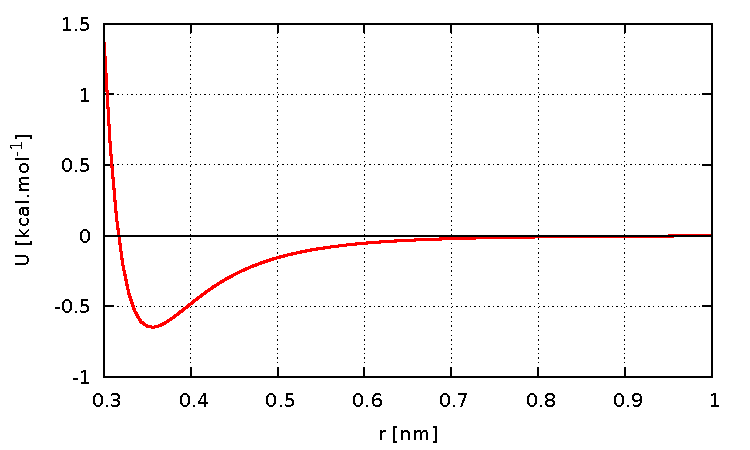
\includegraphics[height = 5 cm]{spce_lj.pdf}
    \caption{Potentiel de Lennard--Jones du modèle \spce{} : {\footnotesize les paramètres de Lennard--Jones sont $A = \qty{0.37122}{(\kilo \cal \per \mol)\tothe{1/6} \nano \meter}$ et $B = \qty{0.3428}{(\kilo \cal \per \mol)\tothe{1/12} \nano \meter}$}}
    \label{fig:spce_lj}
\end{figure}

\begin{table}[h!]
    \centering
    \begin{tabular}{l || c | c}
        \hline
        Caractéristiques               & \reaxff{}         & \spce{}           \\
        \hline
        Modèle de liaisons             & Ordres de liaison & Rigide/Harmonique \\
        Modèle d'angles                & Ordres de liaison & Rigide/Harmonique \\
        Modèle de molécules            & Aucun             & Rigide            \\
        Interactions intermoléculaires & \reaxff{}         & Lennard--Jones    \\
        \hline
    \end{tabular}
    \caption{Comparaison des fonctionnements des modèles}
    \label{tab:comparaison_modeles}
\end{table}

De fait, \reaxff{} est un potentiel objectivement plus flexible que le modèle \spce{} mais implique une charge de calcul beaucoup plus grande.

Par ailleurs, puisque le modèle \spce{} fait appel à des molécules/liaisons/angles rigides, son utilisation avec \lammps{} nécessite l'utilisation d'un format de données de configuration initiale plus complet que \reaxff{}. La conversion des données dans ce format est détaillée à l'\autoref{apdx:conversion_spce}.

\textbf{Mise en place des simulations}\\
Pour faciliter la comparaison des résultats obtenus par simulations aux résultats expérimentaux, les conditions de simulations sont : $T = \qty{300}{\kelvin}, P = \qty{1}{\atm}$.\\
De plus, les simulations suivent un déroulement similaire à celui présenté à la \autoref{sec:deroulement_simulations}, c'est-à-dire :
\begin{itemize}
    \item Une minimisation à \qty{0}{\kelvin}
    \item Une relaxation de \qtyrange{1}{300}{\kelvin} et à \qty{1}{\atm} en \qty{10}{\pico \second}
    \item Une stabilisation de \qty{10}{\pico \second}
    \item La simulation principale pour \qty{1}{\nano \second}
\end{itemize}
et mettent en jeu \num{267} molécules d'eau initialement dans une boîte cubique de côté \qty{20}{\angstrom}.

Les différentes quantités thermodynamiques relevées au cours de ces simulations sont présentées aux \autoref{fig:h2o_relaxation} et \ref{fig:h2o_main}.

Pendant la relaxation et la stabilisation, nous pouvons voir que la température du système augmente progressivement durant les \num{10} premières \unit{\pico \second} avant de se stabiliser à la valeur cible. Quant à l'énergie potentielle, elle diminue abruptement avant de lentement atteindre un plateau.

Pour la simulations principale, il semble que les grandeurs soient équilibrées car elle ne fluctuent plus autant que lors de la relaxation et stabilisation.

\begin{figure}[h!]
    \centering
    \begin{subfigure}{.49\textwidth}
        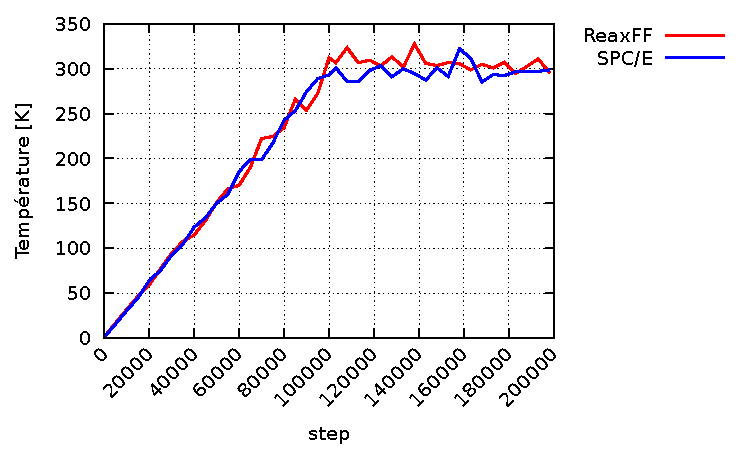
\includegraphics[width = \textwidth]{h2o_relaxation_temp.pdf}
        \caption{Températures}
    \end{subfigure}%
    ~
    \begin{subfigure}{.49\textwidth}
        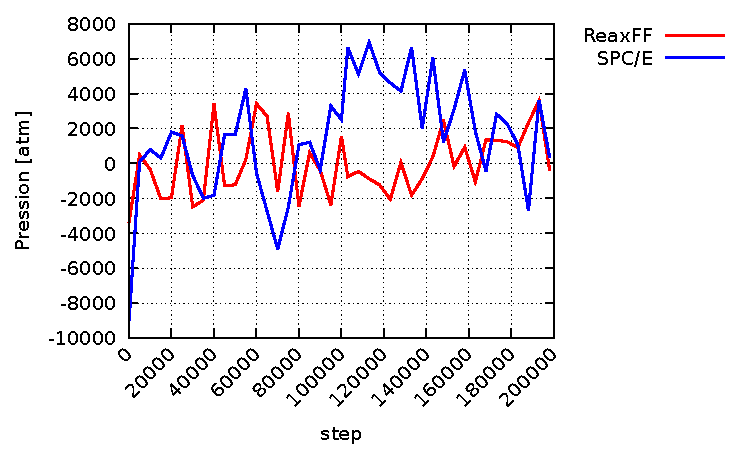
\includegraphics[width = \textwidth]{h2o_relaxation_press.pdf}
        \caption{Pressions}
    \end{subfigure}
    \begin{subfigure}{.49\textwidth}
        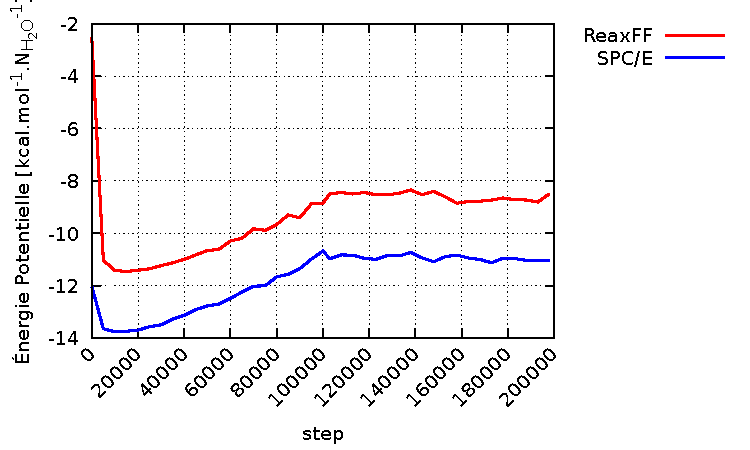
\includegraphics[width = \textwidth]{h2o_relaxation_epot.pdf}
        \caption{Énergies potentielles par molécule}
    \end{subfigure}%
    ~
    \begin{subfigure}{.49\textwidth}
        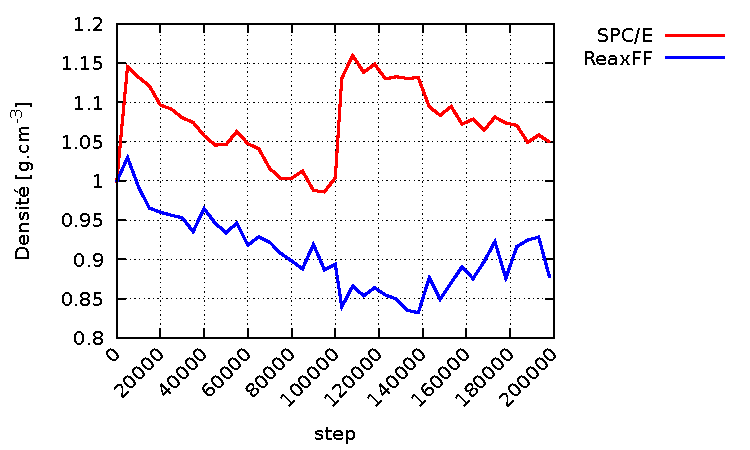
\includegraphics[width = \textwidth]{h2o_relaxation_density.pdf}
        \caption{Densités}
    \end{subfigure}
    \caption{Quantités thermodyanmiques lors de la relaxation}
    \label{fig:h2o_relaxation}
\end{figure}

\begin{figure}[h!]
    \centering
    \begin{subfigure}{.49\textwidth}
        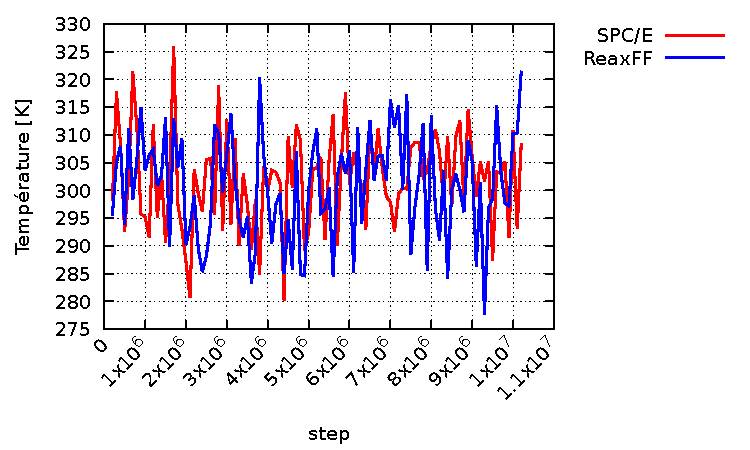
\includegraphics[width = \textwidth]{h2o_main_temp.pdf}
        \caption{Températures}
    \end{subfigure}%
    ~
    \begin{subfigure}{.49\textwidth}
        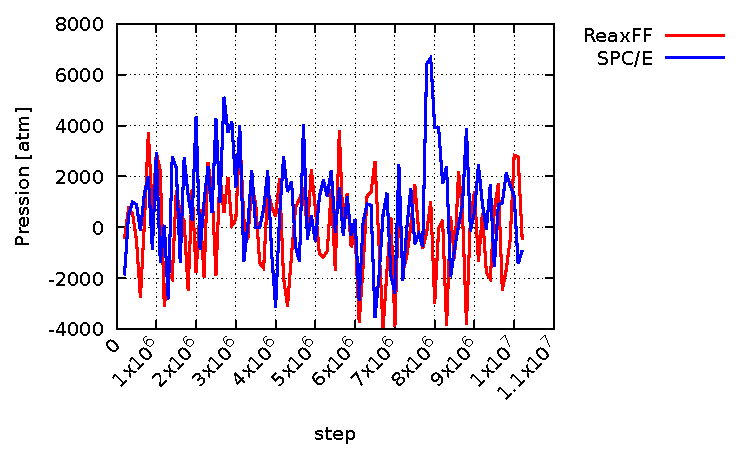
\includegraphics[width = \textwidth]{h2o_main_press.pdf}
        \caption{Pressions}
    \end{subfigure}
    \begin{subfigure}{.49\textwidth}
        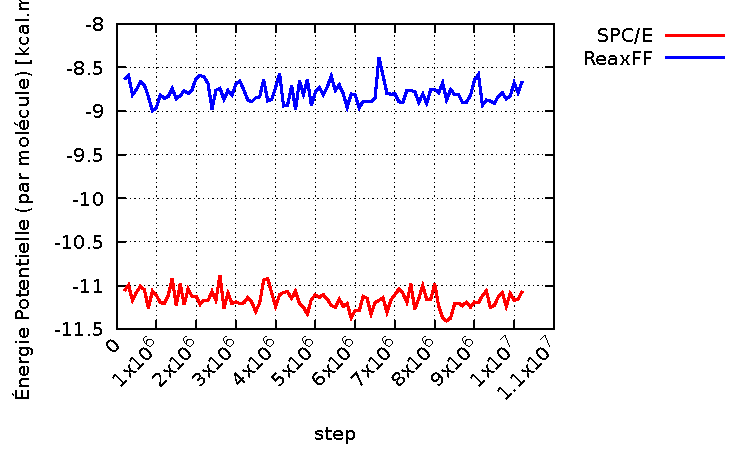
\includegraphics[width = \textwidth]{h2o_main_epot.pdf}
        \caption{Énergies potentielles par molécule}
    \end{subfigure}
    \caption{Quantités thermodynamiques lors de la simulation}
    \label{fig:h2o_main}
\end{figure}

\textbf{Proriétés comparées}\\
Pour cette étude, nous comparons les propriétés structurales et de diffusion des deux modèles avec la \emph{Radial Distribution Function} et le \emph{Mean Squared Displacement}.

En effet, pour rappel, la première des deux grandeurs nous informe sur la probabilité de trouver deux atomes à une distance donnée l'un de l'autre en comparaison à un gaz parfait :
\begin{equation}
    \boxed%
    {
        g (r) = \frac{\left\langle \rho (r) \right\rangle}{\rho} = \frac{\mathrm{d}n(r)}{4 \pi r^2 \mathrm{d}r \rho}
    }
    \label{eq:rdf}
\end{equation}
où $\rho (r)$ est la densité locale de particules, $\left\langle \cdot \right\rangle$ est la moyenne sur l'ensemble, $\mathrm{d}n(r)$ est le nombre de particules à l'intérieur de la coquille sphérique située à $r$ et d'épaisseur $\mathrm{d}r$, et $\rho$ est la densité numérique moyenne de la paire considérée.

Quant à la deuxième quantité, pour des temps sufisamment longs elle nous donne indirectement le coefficient de diffusion du système :
\begin{equation*}
    MSD(t) \equiv \left\langle \left| \vec{r}(t) - \vec{r}(t_0) \right|^2 \right\rangle = 2 d D t
\end{equation*}
où $\vec{r}$ est la position d'une particule, $\left\langle \cdot \right\rangle$ est la moyenne sur l'ensemble, $t_0$ est un temps de référence, $d$ est le nombre de dimensions du problème, $D$ est le coefficient de diffusion du système et $t$ est le temps.

Cependant, pour obtenir une meilleur précision quant au coefficient de diffusion, nous utilisons le \emph{Mean Squared Displacement} moyenné sur les décalages en temps :
\begin{equation}
    \boxed%
    {
        \overline{MSD} (\tau) = \frac{1}{N_{\tau}} \sum_{i = 0}^{N_{\tau}} \left\langle \left| \vec{r}(\tau) - \vec{r}(t_0) \right|^2 \right\rangle  = 2 d D t
    }
\end{equation}
où $\tau$ est un décalage de configurations, et $N_{\tau}$ le nombre de configurations pouvant être décalées de $\tau$ dans la trajectoire. $\overline{MSD}$ est donc, pour chaque décalage de configurations, une moyenne sur l'ensemble de la trajectoire.

\textbf{Résultats obtenus}\\
Nous présentons et discutons des résultats obtenus ci-dessous. Il est important de préciser qu'\textit{a priori} nous attendons des deux modèles une bonne correspondance avec les résultats expérimentaux, c'est-à-dire moins de \qty{15}{\percent} d'erreurs relatives ; Et cela car d'un côté \spce{} est un modèle exclusivement conçu pour la molécule d'eau et de l'autre \reaxff{} se base sur des résultats très précis issus de simulations \textit{ab initio}.

Les résultats obtenus à l'issue des simulations sont comparées aux valeurs expérimentales correspondantes\cite{soper_radial_2000}\cite{tsimpanogiannis_self-diffusion_2019} (\autoref{tab:h2o_rdf} et \ref{tab:h2o_diffusion}).

\begin{table}[h!]
    \centering
    \begin{tabular}{l | c c | c c}
        \hline
        Données &1\textsuperscript{er} max. [\unit{\angstrom}] &$g$\textsubscript{\ce{OH}} &2\textsuperscript{e} max. [\unit{\angstrom}] &$g$\textsubscript{\ce{OH}}\\
        \hline
        Expérimentale\cite{soper_radial_2000} &\num{0.93} &\num{11.66} &\num{1.80} &\num{1.15}\\
        \reaxff{} &\num{0.94} &\num{22.18} &\num{1.84} &\num{1.35}\\
        \spce{} &\num{1.00} &\num{23.99} &\num{1.72} &\num{1.71}\\
        \hline
    \end{tabular}
    \begin{tabular}{c c | c c}
        \hline
        1\textsuperscript{er} max. [\unit{\angstrom}] &$g$\textsubscript{\ce{OO}} &2\textsuperscript{e} max. [\unit{\angstrom}] &$g$\textsubscript{\ce{OO}}\\
        \hline
        \num{2.74} &\num{2.94} &\num{4.45} &\num{1.18}\\
        \num{2.83} &\num{2.78} &\num{4.45} &\num{1.20}\\
        \num{2.76} &\num{3.14} &\num{4.44} &\num{1.16}\\
        \hline
    \end{tabular}
    \caption{Résultats pour les \emph{Radial Distribution Function}s}
    \label{tab:h2o_rdf}
\end{table}

\begin{table}[h!]
    \centering
    \begin{tabular}{l || c | c}
        \hline
        Données &Coefficient de diffusion (\unit{\square \meter \per \second}) &Erreur relative (\unit{\percent})\\
        \hline
        Expérimentale\cite{tsimpanogiannis_self-diffusion_2019} &\num{2.30e-9} &--\\
        \reaxff{} &\num{2.45e-9} &\num{6.5}\\
        \spce{} &\num{1.61e-9} &\num{30}\\
        \hline
    \end{tabular}
    \caption{Résultats pour les coefficients de diffusion}
    \label{tab:h2o_diffusion}
\end{table}

Pour les \emph{Radial Distribution Function}s, nous comparons les pics que nous jugeons les plus importants, c'est-à-dire :
\begin{itemize}
    \item l'abscisse du premier maximum de $g_{\ce{OH}}$ donnant des indications sur la longueur de la liaison \ce{OH} ; L'intensité des pics n'est pas prise en compte car elle trop sensible à la valeur de la largeur $\mathrm{d}r$ et à la précision du calcul de la $g_{\ce{OH}}$
    \item le second maximum de la $g_{\ce{OH}}$, caractéristique des liaisons hydrogène de la molécule d'eau
    \item le premier maximum de la $g_{\ce{OO}}$, indicateur des distances intermoléculaires (notamment pour \spce{})
    \item le second maximum de la $g_{\ce{OO}}$
\end{itemize}

\reaxff{} a de meilleurs résultats que le modèle \spce{} pour l'abscisse du premier pic de la $g_{\ce{OH}}$ [\qty{1.1}{\percent} contre \qty{7.5}{\percent}], pour le second pic de la $g_{\ce{OH}}$ [\qty{2.2}{\percent} contre \qty{4.4}{\percent} en absicce ; \qty{17.4}{\percent} contre \qty{48.7}{\percent} en intensité], pour l'intensité du premier pic de la $g_{\ce{OO}}$ [\qty{5.4}{\percent} contre \qty{6.8}{\percent}], et pour l'abscisse du second pic de la $g_{\ce{OO}}$ où il correspond exactement à la valeur expérimentale.

De l'autre côté, le modèle \spce{} a de meilleurs résultats que \reaxff{} pour l'abscisse du premier pic de la $g_{\ce{OO}}$ [\qty{0.7}{\percent} contre \qty{3.3}{\percent}].

Enfin, les modèles ont la même erreur pour l'intensité du second pic de la $g_{\ce{OO}}$ [\qty{1.7}{\percent}].

\begin{figure}[h!]
    \centering
    \begin{subfigure}{\textwidth}
        \centering
        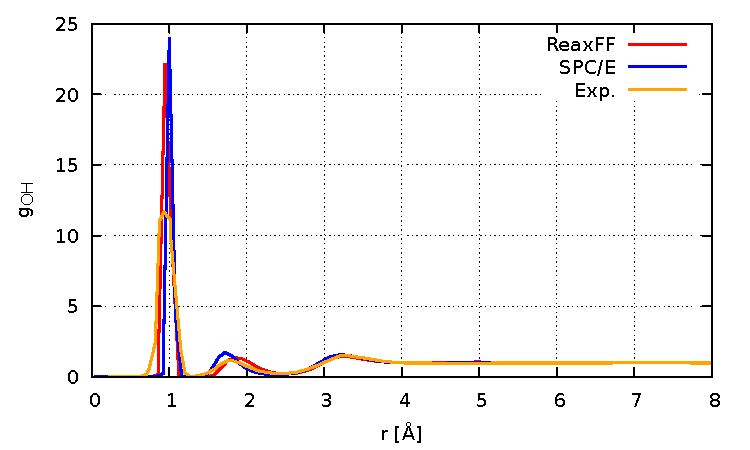
\includegraphics[width = \textwidth]{h2o_rdf_oh.pdf}
        \caption{Pour la paire \ce{OH} : \reaxff{} a de meilleurs résultats que \spce{} sur tous les points, cependant les deux modèles présentent de grandes erreurs pour l'intensité du second pic}
        \label{fig:h2o_rdf_oh}
    \end{subfigure}

    \begin{subfigure}{\textwidth}
        \centering
        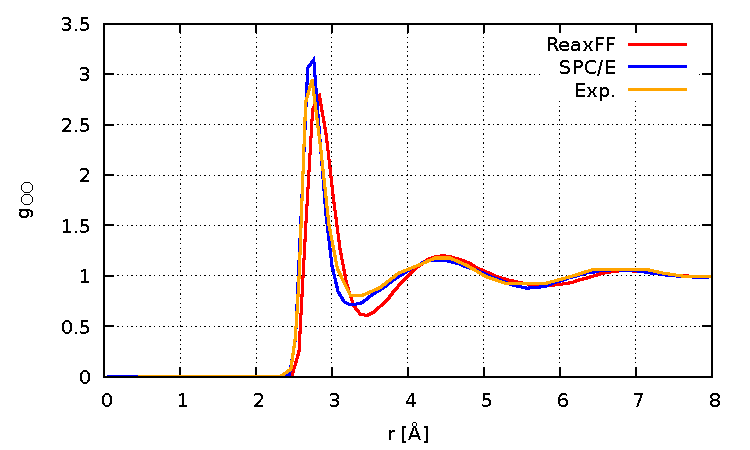
\includegraphics[width = \textwidth]{h2o_rdf_oo.pdf}
        \caption{Pour la paire \ce{OO} : \spce{} représente mieux l'abscisse du premier pic mais \reaxff{} a une erreur moindre quant à son intensité ; Les deux modèles ont de bons résultats pour le second pic}
        \label{fig:h2o_rdf_oo}
    \end{subfigure}
    \caption{Comparaison des \emph{Radial Distribution Function}s : même si les erreurs relatives restent globalement correctes, \reaxff{} a plus souvent de meilleurs résultats par rapport aux points comparés}
    \label{fig:h2o_comparaison_resultats}
\end{figure}

\begin{figure}[h!]
    \centering
    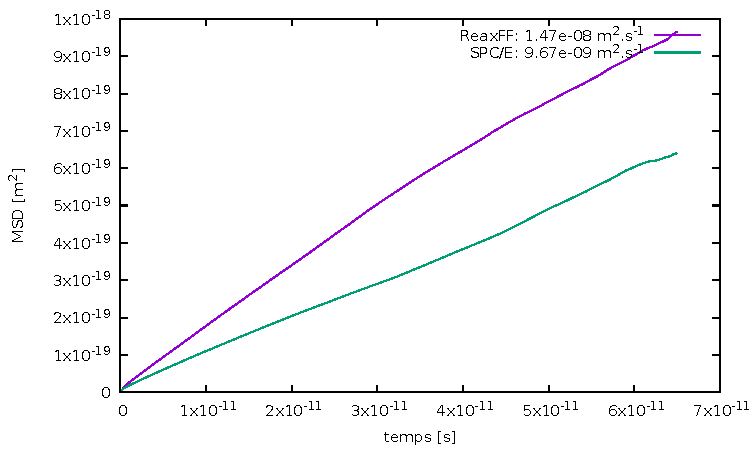
\includegraphics[width = \textwidth]{h2o_msd.pdf}
    \caption{Comparaison des \emph{Mean Squared Displacement}s : les coefficients de diffusion sont calculés avec les pentes de ces courbes ; Pour les deux courbes on a $R = 0.99$}
    \label{fig:h2o_msd}
\end{figure}

Pour les \emph{Mean Squared Displacement}s, \reaxff{} modélise mieux la diffusion que le modèle \spce{} [\qty{6.5}{\percent} contre \qty{30}{\percent}]. Nous pouvons supposer que cette grande différence est due au fait que le modèle \spce{} n'a pas été pensé pour représenter la diffusion de la molécule mais sa polarité.
